\documentclass[serif, xcolor={svgnames, table}, usepdftitle=false]{beamer}

\usetheme{Warsaw}

% Fonts
\usepackage{fontspec}

% Languages and bibliographies
\usepackage{polyglossia}
\usepackage{csquotes}
\usepackage[hyperref, backref, backend=biber]{biblatex}

% Mathematics
\usepackage{mathtools}
\usepackage[math-style=TeX, bold-style=upright]{unicode-math}
\usepackage{stmaryrd}

% Pseudocode
\usepackage{algorithm}
\usepackage{algpseudocode}
\usepackage{varwidth}

% Microtype
\usepackage{microtype}

% Graphics and captioning
\usepackage{graphicx}
\usepackage{caption}
\usepackage{subcaption}

% Tables
\usepackage{booktabs}

% Numbers
\usepackage{siunitx}
\usepackage{nth}

%
% Package setup
%

\setmainlanguage{english}
\setmathfont{Latin Modern Math}
\mathtoolsset{mathic=true}
\sisetup{%
  detect-all,
  detect-display-math,
  binary-units
}

\addbibresource{Bibliography.bib}

\hypersetup{%
  unicode,
  pdfinfo={%
    Title={Queueing Networks},
    Subject={Teletraffic Engineering},
    Author={Dario Gjorgjevski},
    Keywords={Teletraffic Engineering, Network Planning, Queueing Theory}
  }
}

\renewcommand*{\vec}{\symbf}
\newcommand*{\mat}{\symbf}
\DeclarePairedDelimiter\abs{\lvert}{\rvert}
\DeclarePairedDelimiter\norm{\lVert}{\rVert}

\graphicspath{{Figures/}}

%
% Title
%

\title{Queueing Networks}
\subtitle{Teletraffic Engineering and Network Planning}
\author[Dario Gjorgjevski]{Dario Gjorgjevski\inst{1}\\
  \texttt{\href{mailto:gjorgjevski.dario@students.finki.ukim.mk}
    {gjorgjevski.dario@students.finki.ukim.mk}}}
\institute[FCSE]{\inst{1}Faculty of Computer Science and Engineering\\
  Ss.\ Cyril and Methodius University in Skopje}
\date{May 26, 2016}

%
% Logo
%

\logo{
\includegraphics[height=0.66cm]{Logo.png}}

\begin{document}

\AtBeginSection[]{%
  \begin{frame}{Outline}
    \tableofcontents[currentsection]
  \end{frame}
}

\begin{frame}
  \titlepage
\end{frame}

\section{Introduction}

\subsection{Motivation and basic definitions}

\begin{frame}{The motivation behind queueing networks}
  \begin{itemize}
  \item In real systems, jobs often receive service from multiple successive
    nodes.
  \item The total service demand is composed of demand at all these nodes.
  \item Hence, we have a network of queues -- a \emph{queueing network}.
  \item Arrival process at one queue is a departure process at another queue and
    vice-versa.
  \end{itemize}
\end{frame}

\begin{frame}{Basic definitions to remember}
  \only<1>{%
    \begin{itemize}
    \item The queueing network is composed of individual queues, each called a
      \emph{node}.
    \item The total number of jobs (incl.\ delayed and served jobs) at a node is
      called the \emph{queue length}.
    \item Similarly, the \emph{waiting (sojourn)} time includes both the
      \emph{delay} and the \emph{service} times.
    \item Two types of queueing networks:
      \begin{itemize}
      \item \emph{Closed} -- fixed number of ``customers;'' and
      \item \emph{Open} -- varying number of ``customers.''
      \end{itemize}
    \end{itemize}
  }
  \only<2>{%
    \begin{itemize}
    \item $M/M/n$ is a classical example of an open network.
    \item Palm's machine-repair model is a classical example of a closed network.
    \item More types of customers can lead to a network being \emph{both} open and
      closed.
    \item Describe the state by $p(x_1, \ldots, x_K)$, $x_k$ is the number of
      customers at node $k$ ($k = 1, \ldots, K$).
    \item Every node is reversible $\implies$ $p(x_1, \ldots, x_K)$ can be
      written as a product form.
    \end{itemize}
  }
\end{frame}

\subsection{Customer types}

\begin{frame}{Considering multiple types of customers}
  \begin{itemize}
  \item Multiple types of customers, each forming a \emph{chain}.
  \end{itemize}
  \begin{figure}[!h]
    \centering
    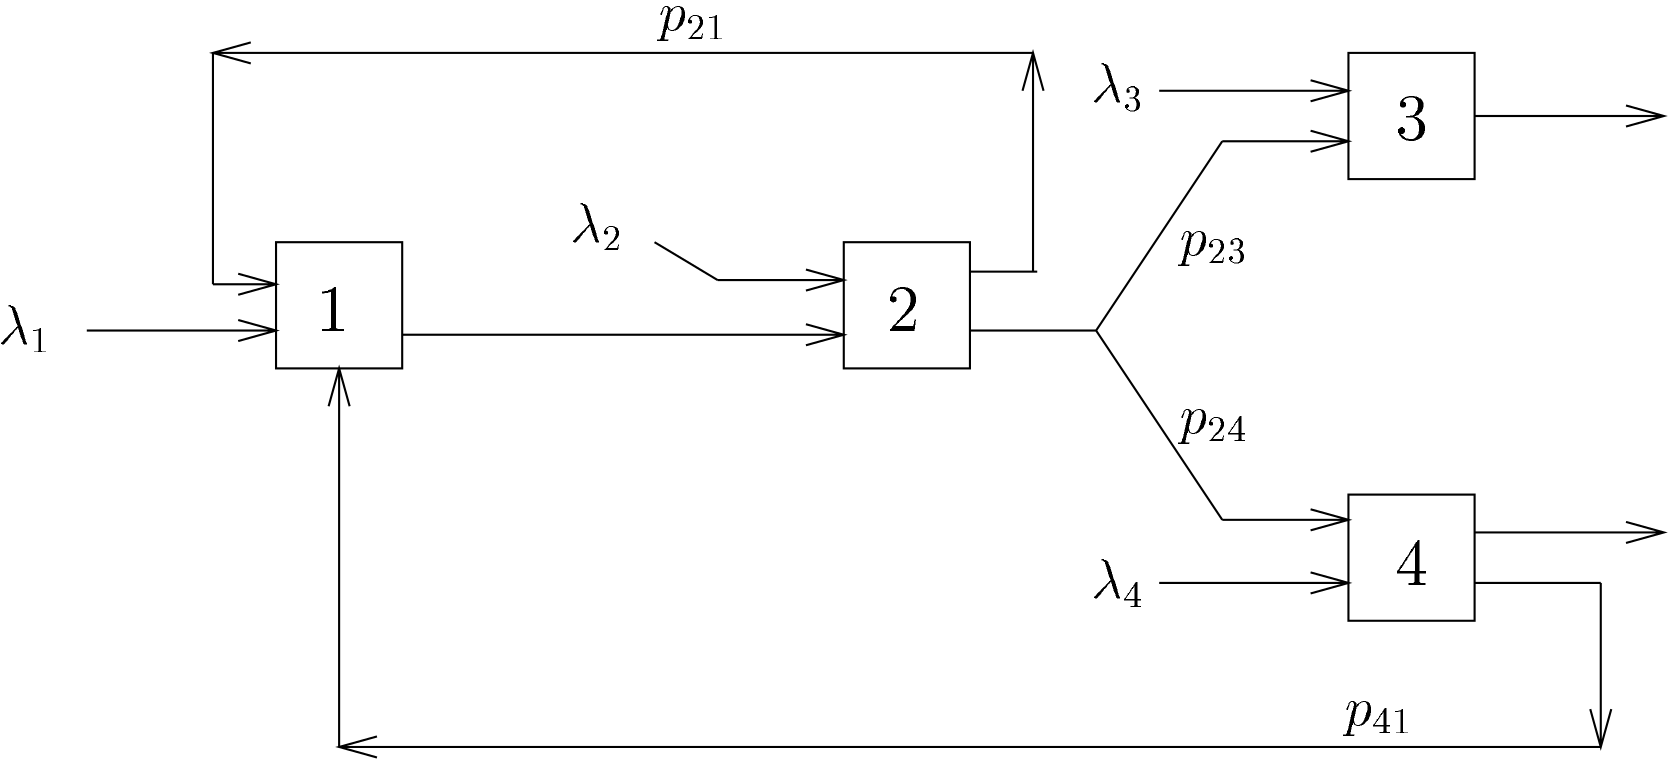
\includegraphics[width=\linewidth]{Chains.png}
    \caption{A queueing network with four chains}
  \end{figure}
\end{frame}

\section{Reversible queueing systems}

\subsection{Preliminaries}

\begin{frame}{What is reversibility?}
  Running the queue ``backwards in time'' gives the same queue.

  \begin{definition}[Reversibility]
    A queue is reversible if and only if there is no circulation flow, i.e., the
    circulation flow among four neighboring states in a square equals $0$.
  \end{definition}

  Kolmogorov's cycle criterion proves that this is a necessary and sufficient
  condition for a queue (or more generally, a Markov process) to be reversible.
\end{frame}

\begin{frame}{The importance of reversibility}
  \begin{itemize}
  \item Reversibility means that the departure process is the same as the
    arrival process.
  \item In other words, if the arrival process is Poisson, so is the departure.
  \end{itemize}
  $\implies$ This simplifies things greatly.
\end{frame}

\subsection{State probabilities for reversible systems}

\begin{frame}{The $M/M/n$ case}
  \begin{theorem}[Burke]
    The departure process of an $M/M/n$ system is a Poisson process.  The state
    probabilities are given by
    \begin{equation*}
      \frac{p(x)}{p(0)} =
      \begin{cases}
        \frac{A^x}{x!} & \text{if }0\le x \le n \\
        \frac{A^x}{n! n^{x - n}} & \text{if }x > n\text{,}
      \end{cases}
    \end{equation*}
    where $A = \lambda / {\mu}$ and $p(0)$ is found by solving for normalization
    conditions.
  \end{theorem}
\end{frame}

\begin{frame}{Other cases}
  Other well known cases ($M/M/1$, $\text{IS}$, $M/G/1\text{-PS}$,
  $M/G/n \text{-GPS}$, $M/G/1\text{-LCFS-PR}$) have also been proven to have
  Poisson departure processes.

  \begin{example}[$M/M/1$]
    It may seem counter-intuitive that the departure process of an $M/M/1$
    system with arrival rate $\lambda$ and service rate $\mu$ is a Poisson
    process with rate $\lambda$.  However, decomposing the departure process
    into Cox-distributions where one branch corresponds to idle, and the other
    to busy periods provides a nice graphical proof.
  \end{example}
\end{frame}

\section{Open networks}

\subsection{Single chain}

\begin{frame}{The setup we will be looking at}
  \begin{itemize}
  \item Each node is an $M/M/n$ system with $n_k$ servers and $\mu_k$ service
    rate.
  \item Jobs arrive at node $k$ according to a Poisson process with rate
    $\lambda_k$.
  \item Jobs may arrive at node $k$ from other nodes.
  \item A job leaving node $j$ is transferred to $k$ with probability $p_{j k}$
    or leaves the network with probability $1 - \sum\nolimits_{k = 1}^{K} p_{j
      k}$.
  \end{itemize}
\end{frame}

\begin{frame}{Calculating the arrival intensity}
  \begin{itemize}
  \item Solve the balance equations to calculate for the arrival rates at each
    node $k$:
    \begin{equation}
      \Lambda_k = \lambda_k + \sum\limits_{j = 1}^{K} \Lambda_j p_{j k }\text{.}
    \end{equation}
  \item Assume
    \begin{equation*}
      \frac{\Lambda_k}{\mu_k} = A_k \le n_k\text{,}
    \end{equation*}
    otherwise queue length $\to \infty$.
  \end{itemize}
\end{frame}

\begin{frame}{Jackson's theorem}
  \begin{theorem}[Jackson~\autocite{Jac57}]
    Under the aforementioned setup,
    $$
    p(x_1, \ldots, x_K) = \prod\limits_{k = 1}^{K} p_k(x_k)\text{.}
    $$
  \end{theorem}

  In other words, we can consider each node independently with state
  probabilities as in Erlang's delay system ($M/M/n$).
\end{frame}

\begin{frame}{Performance measures}
  \begin{itemize}
  \item
    $\displaystyle \text{Total throughput} = \Lambda = \sum\limits_{k = 1}^{K}
    \Lambda_k$.
  \item $\displaystyle \text{Average load at node }k = \frac{\Lambda_k}{\mu_k}$.
  \item $\displaystyle \text{Visits to node }k = \frac{\Lambda_k}{\Lambda}$.
  \item
    $\displaystyle \text{Average \# of jobs at node }k = N_k = \sum\limits_{n
      = 0}^{\infty} n p_k(n)$.
  \item
    $\displaystyle \text{Mean sojourn time} = \sum\limits_{k = 1}^{K}
    \frac{N_k}{\Lambda}$.
  \end{itemize}
\end{frame}

\subsection{Multiple chains}
\begin{frame}{Reducing multiple chains to a single chain}
  \begin{itemize}
  \item Solve the flow balance equations for each chain, obtaining the arrival
    intensity from chain $j$ to node $k$ ($\Lambda_{j k}$).
  \item Exploit local balance to solve for the state probabilities.
  \item Apply Jackson's theorem.
  \end{itemize}
\end{frame}

\section{Closed networks}
\subsection{Buzen's convolution algorithm}
\begin{frame}{Initial thoughts on closed networks}
  \begin{itemize}
  \item Assume $S$ customers are circulating within $K$ nodes.
  \item Handling closed networks is very complex as we don't know the true
    arrival rate.
  \item We are again interested in $p(x_1, \ldots, x_K)$.
  \item Knowing the arrival rate at a single node lets us solve the balance
    equations for the relative arrival rates to other nodes.
  \item Relative rates still need to be normalized:
    $\displaystyle \binom{S + K - 1}{K - 1}$ terms to sum over naively.
  \item Buzen's convolution algorithm lets us do the normalization in
    $\mathcal{O}(S K)$ time.
  \end{itemize}
\end{frame}

{\setbeamertemplate{logo}{}%
  \begin{frame}{The Gordon--Newell theorem}
    \begin{theorem}[Gordon--Newell~\autocite{GN67}]
      In a closed networks with $S$ customers and $K$ nodes with arrival rates
      $\Lambda_k$,
      \begin{equation*}
        p(x_1, \ldots, x_K) = \frac{1}{G(S)} \prod\limits_{k = 1}^{K}
        \left(\frac{\Lambda_k}{\mu_k}\right)^{x_k}\text{,}
      \end{equation*}
      where the $\Lambda_k$ are found by solving the balance equations and $G(S)$
      is a normalization constant:
      \begin{equation*}
        G(S) = \sum\limits_{(x_1,\ldots,x_K)} \prod\limits_{k = 1}^{K} \left(\frac{\Lambda_k}{\mu_k}\right)^{x_k}\text{.}
      \end{equation*}
    \end{theorem}
  \end{frame}}

\begin{frame}{Calculating $G(S)$}{\emph{The} convolution algorithm}
  We can exploit the structure of the network to calculate $G(S)$ relatively
  efficiently~\autocite{Buz73}.
  \begin{enumerate}
  \item Consider each node individually as if offered PCT-I traffic $a_k =
    \frac{\Lambda_K}{\mu_k}$, and calculate the relative state probabilities
    $q_k(x_k)$.
  \item Convolve the probabilities of the nodes recursively, e.g.,
    \begin{equation*}
      q_{1,\ldots,i,\ldots,k} = q_{1,\ldots,i - 1,i + 1,\ldots,k} \ast q_i\text{.}
    \end{equation*}
  \end{enumerate}
  The above procedure terminates as soon as $q_{1, \ldots, K}$ has been
  computed.  It can be shown that $G(S) = q_{1, \ldots, K}$.
\end{frame}

\begin{frame}{An example of applying the convolution algorithm}
  \begin{example}[Palm's machine-repair model]
    Assume a computer system with $S$ jobs and terminals, and one server.  The
    \emph{mean thinking time} is $\mu_1^{-1}$, and the \emph{mean service time}
    is $\mu_2^{-1}$.  In other words, there are two nodes: the terminals and the
    server.  The relative loads are $a_1 = \Lambda / {\mu_1}$ and
    $a_2 = \Lambda / {\mu_2}$.

    By convolving $q_1(i)$ and $q_2(j)$, we get
    \begin{align*}
      q_{1, 2}(S) &= (q_1 \ast q_2)(S) \\
                  &= a_1^0 a_2^S + a_1^1 a_2^{S - 1} + \frac{a_1^2}{2!} a_2^{S -
                    2} + \ldots + \frac{a_1^S}{S!} a_2^0\text{.}
    \end{align*}
  \end{example}
\end{frame}

\begin{frame}{Palm's machine-repair model}
  The probability that all terminals are thinking is identified as
  $\frac{q_1(S) q_2(0)}{q_{1, 2}(S)}$, which agrees with Erlang's B-formula.
  \begin{figure}[!h]
    \centering
    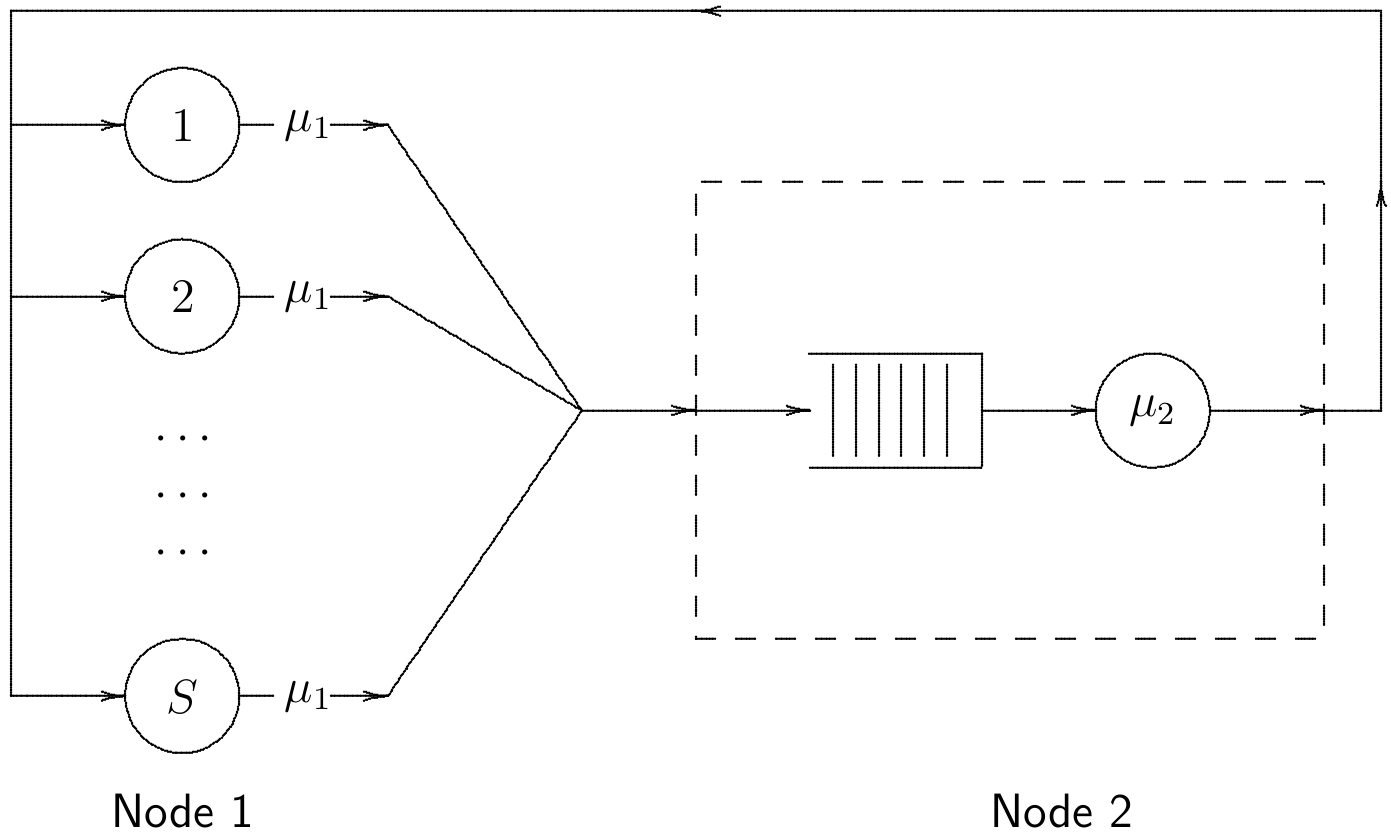
\includegraphics[width=\textwidth, height=0.6\textheight,
    keepaspectratio]{Palm.png}
    \caption{Palm's machine-repair model}
  \end{figure}
\end{frame}

\begin{frame}{The full calculation in Palm's machine-repair model}
  \begin{table}
    \centering
    \newcolumntype{C}{>{$ \displaystyle}c<{$}}
    \caption{The algorithm applied to Palm's machine-repair
      model}\label{tbl:conv-ex}
    \begin{tabular}{C C C C}
      \toprule
      x & q_1(x_1) & q_2(x_2) & q_{1, 2}(x) = (q_1 \ast q_2)(x) \\
      \midrule
      0 & 1 & 1 & 1 \\
      1 & a_1 & a_2 & a_1 + a_2 \\
      2 & \frac{a_1^2}{2!} & a_2^2 & a_2^2 + a_1 a_2 + \frac{a_1^2}{2!} \\
      \vdots & \vdots & \vdots & \vdots \\
      x & \frac{a_1^x}{x!} & a_2^x & \vdots \\
      S & \frac{a_1^S}{S!} & a_2^S & q_{1, 2}(S) \\
      \bottomrule
    \end{tabular}
  \end{table}
\end{frame}

\subsection{The mean-value algorithm (MVA)}
\begin{frame}{Preliminaries for the MVA}
  We will state two theorems that the MVA uses.

  \begin{theorem}
    For fully accessible systems with a limited number of sources, a random
    source will, upon arrival, observe the system as if the source itself does
    not belong to it.
  \end{theorem}

  \begin{theorem}[Little]
    The mean queue length is equal to call intensity multiplied by the mean
    waiting time, i.e.,
    \begin{equation*}
      L = \lambda  W\text{.}
    \end{equation*}
  \end{theorem}
\end{frame}

\begin{frame}{Definition of the MVA}
  \begin{itemize}
  \item Let the average number of customers at node $k$ be $L_k(S)$.
  \item Obviously, $\sum\nolimits_{k = 1}^{K} L_k(S) = S$.
  \item Now, proceed in two steps:
    \begin{enumerate}
    \item Increase $S$ to $S + 1$.  The average sojourn times become
      $W_k(S + 1) = (L_k(S) + 1) \mu_k^{-1}$ or $\mu^{-1}$, for $1$ and $\infty$
      servers respectively.
    \item By Little's theorem, $L_k(S + 1) = c \lambda_k W_K(S + 1)$, where $c$
      is a normalizing constant.
    \end{enumerate}
  \end{itemize}

  These two steps allow us to compute performance measures efficiently.  Note
  that the results are only approximate for multi-server systems.
\end{frame}

\subsection{BCMP networks}
\begin{frame}{Defining BCMP networks}
  \begin{itemize}
  \item So far, when dealing with closed networks, we assumed a single chain.
  \item In 1975, Baskett, Chandy, Muntz, and Palacios showed that even closed
    networks with multiple chains admit product form solutions if they have
    either:
    \begin{itemize}
    \item FCFS with exponential service times;
    \item Processor sharing queues;
    \item Infinite server queues;
    \item LCFS with pre-emptive resume.
    \end{itemize}
  \item In the last three cases, service time distributions must have rational
    Laplace transforms.
  \item Simple extensions to the convolution and mean-value algorithms.
  \end{itemize}
\end{frame}

\begin{frame}{References}
  \printbibliography[heading=none]
\end{frame}

\begin{frame}[plain, c]
  \begin{center}
    FIN

    Feel free to ask questions.
  \end{center}
\end{frame}
\end{document}

%%% Local Variables:
%%% mode: latex
%%% fill-column: 80
%%% TeX-command-extra-options: "-shell-escape"
%%% TeX-engine: luatex
%%% TeX-master: t
%%% End: